\section{Theoretische Grundlagen}

    \subsection{Zielsetzung}

        \noindent In diesem Versuch werden allgemeine Relaxionsverhalten und vor allem am RC-Kreis untersucht.

    \subsection{Allgemeine Relaxionsgleichung}

        \noindent Eine Relaxion beschreibt das Verhalten wenn ein System angeregt wird und dann wieder nicht-oszillatorisch in seinen 
        Ausgangszustand zurückkehrt. Die Geschwindigkeit mit dem dies passiert ist die Ableitung der Physikalischen Größe $A$ ist zumeist 
        proportional zur aktuellen Auslenkung vom Ausgangszustand der wieder bei $A(\infty)$ erreicht wird:

        \begin{equation}
            \frac{\symup{d}A}{\symup{d}t}=c[A(t)-A(\infty)]
            \label{eqn:1}
        \end{equation}

        \noindent Die Integration dieser Gleichung:

        \begin{equation*}
            \int_{A(0)}^{A(t)} \frac{\symup{d}A'}{A' - A(\infty)} = \int_0^t \symup{d}t'
        \end{equation*}

        \noindent liefert

        \begin{equation*}
            \text{ln} \frac{A(t) - A(\infty)}{A(0) - A(\infty)} = ct
        \end{equation*}

        \noindent oder

        \begin{equation}
            A(t) = A(\infty) + [A(0) - A(\infty)] \text{e}^{ct} . 
            \label{eqn:2}
        \end{equation}

        \noindent Hier muss $c < 0$ sein damit $A(t)$ konvergiert.

    \subsection{Entladevorgang im RC-Kreis}

        \noindent Das Standardbeispiel für Relaxionsverhalten in der Physik sind das Aufladen und Entladen eines Kondensators über einen 
        Widerstand(siehe Abbildung \ref{img:A_und_e}).

        \begin{figure}
            \centering
            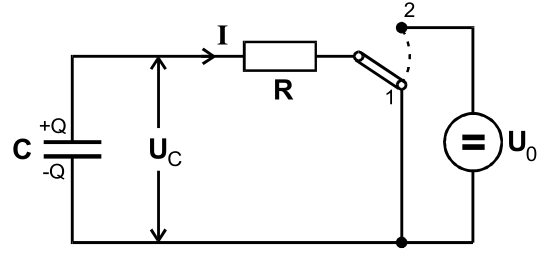
\includegraphics[width=0.70\textwidth]{latex/images/Auflade_und_entlade.PNG}
            \caption{Entladung(1) und Aufladung(2) eines RC-Kreises.\protect \cite{V353}.}
            \label{img:A_und_e}
        \end{figure}

        \noindent Zum Entladen schauen wird wie in Abbildung \ref{img:A_und_e} ein Kondensator mit Kapazität $C$ mit der Ladung $Q$ betrachtet.
        Damit ergibt sich die Kondensatorspannung $U_C$ zu:

        \begin{equation}
            U_{\text{C}} = \frac{Q}{C}
            \label{eqn:3}
        \end{equation}

        \noindent damit berechnet sich nach dem ohmschen Gesetz die Stromstärke durch einen Widerstand $R$ zu

        \begin{equation}
            I = \frac{U_{\text{C}}}{R} .
            \label{eqn:4}
        \end{equation}

        \noindent Auf einem Zeitintervall d$t$ ändert sich die Ladung auf dem Kondensator somit um den Wert:

        \begin{equation}
            \text{d}Q = -I \text{d}t
            \label{eqn:5}
        \end{equation}

        \noindent Über die Gleichungen (\ref{eqn:3}), (\ref{eqn:4}) und (\ref{eqn:5}) lässt sich nun eine Differential Gleichung für die 
        Ladung auf dem Kondensator aufstellen:

        \begin{equation}
            \frac{\text{d}Q}{\text{d}t} = - \frac{1}{RC} Q(t).
            \label{eqn:DGL}
        \end{equation}

        \noindent Da die Ladung auf dem Kondensator für große Zeit gegen 0 konvergiert hat die DGL()\ref{eqn:DGL}) die Form der 
        Gleichung(\ref{eqn:1}). Nach Gleichung(\ref{eqn:2}) ergibt die Integration

        \begin{equation*}
            Q(t) = Q(0) \text{exp}(-t/RC).
        \end{equation*}

    \subsection{Aufladevorgang im RC-Kreis}

        \noindent Analog zum Entladevorgang lässt sich eine Gleichung für den Aufladevorgang aufstellen. Hier ist der Kondensator über einen 
        Widerstand $R$ an eine Spannungsquelle der Spannung $U_0$ angeschlossen. Die Randbedingungen ergeben sich somit zu:
    
        \begin{equation}
            Q(0) = 0 \quad \text{und} \quad Q(\infty) = CU_0 
        \end{equation}

        \noindent Der Aufladevorgang kann somit durch 

        \begin{equation}
            Q(t) = CU_0(1- \text{exp}(-t/RC))
        \end{equation}

        \noindent beschrieben werden. Hier wird der Ausdruck $RC$ als Zeitkonstante bezeichnet. Sie gibt an mit welcher Geschwindigkeit 

        \begin{equation}
            \frac{Q(t = RC)}{Q(0)} = \frac{1}{e} \approx 0,368
        \end{equation}

        \begin{equation}
            U(t) = U_0 \text{cos}( \omega t)
        \end{equation}

        \begin{equation}
            U_{\text{C}}(t) = A(\omega) \text{cos}(\omega t + \varphi \{ \omega \} )
        \end{equation}

        \begin{equation}
            U(t) = U_R(t) + U_C(t)
        \end{equation}

        \begin{equation}
            U_0 \text{cos}(\omega t) = I(t)R + A(\omega) \text{cos}(\omega t + \varphi)
        \end{equation}

        \begin{equation}
            I(t) = \frac{\text{d}Q}{\text{d}t} = C \frac{\text{d}U_\text{C}}{\text{d}t}
        \end{equation}

        \begin{equation}
            U_0 \text{cos}(\omega t) = -A\omega R C \text{sin}(\omega t + \varphi) + A(\omega) \text{cos}(\omega t + \varphi)
        \end{equation}

        \begin{equation}
            0 = -\omega R C \text{sin} \left( \frac{\pi}{2} + \varphi \right) + \text{cos} \left( \frac{\pi}{2} + \varphi \right)
        \end{equation}

        \begin{equation}
            \frac{\text{sin} \varphi}{\text{cos} \varphi} = \text{tan} \varphi (\omega) = -\omega RC 
        \end{equation}

        \begin{equation}
            \varphi (\omega) = \text{arctan} ( - \omega R C)
        \end{equation}

        \begin{equation}
            \omega t + \varphi = \frac{\pi}{2}
        \end{equation}

        \begin{equation}
            U_0 \text{cos}(\frac{\pi}{2} - \varphi) = -A \omega R C 
        \end{equation}

        \begin{equation}
            A(\omega) = - \frac{\text{sin} \varphi}{\omega R C} U_0
        \end{equation}

        \begin{equation}
            \text{sin}^2 \varphi + \text{cos}^2 \varphi = 1
        \end{equation}

        \begin{equation}
            \text{sin} \varphi = \frac{\omega R C}{ \sqrt{1 + \omega^2 R^2 C^2} }
        \end{equation}

        \begin{equation}
            A(\omega) = \frac{U_0}{\sqrt{1 + \omega^2 R^2 C^2}}
        \end{equation}

        \begin{equation}
            U(t) = U_{\text{R}}(t) + U_{\text{C}}(t) = I(t) \cdot R + U_{\text{C}}(t)
        \end{equation}

        \begin{equation}
            U(t) = RC \frac{\text{d}U_{\text{C}}}{\text{d}t} + U_{\text{C}}(t)
        \end{equation}

        \begin{equation}
            U(t) = RC \frac{\text{d}U_{\text{C}}}{\text{d}t}
        \end{equation}

        \begin{equation}
            U_{\text{C}}(t) = \frac{1}{RC} \int_0^t U(t')\text{d}t'
        \end{equation}